%&tex
\documentclass{standalone}

\usepackage[dvipsnames]{xcolor}

\usepackage{tikz}
\usetikzlibrary{positioning}

\begin{document}

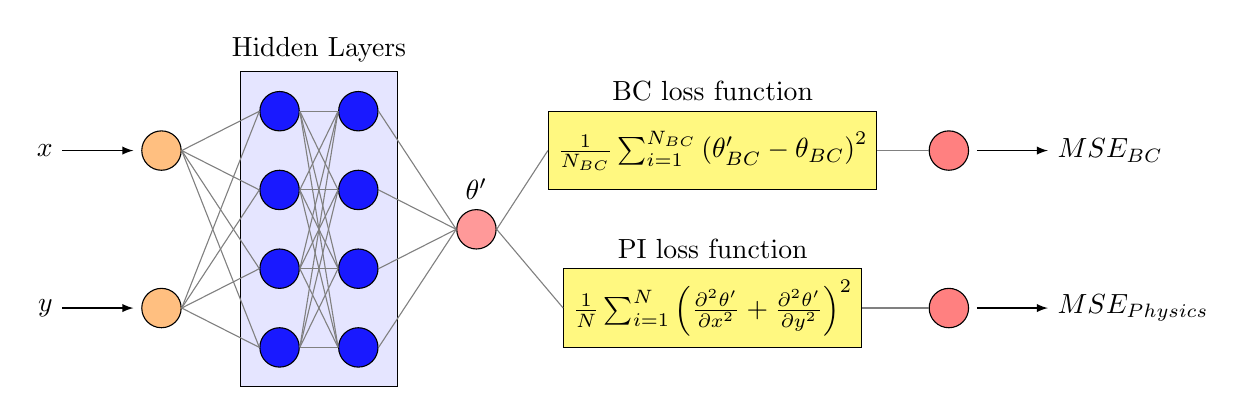
\begin{tikzpicture}
    % input layer nodes
    \node[draw,
    circle,
    minimum size = 0.5cm,
    fill=orange!50] (X) at (0,1) {};
    \node[draw,
    circle,
    minimum size = 0.5cm,
    fill=orange!50] (Y) at (0,-1) {};

    % hidden layer cover
    \node[draw,
    rectangle,
    minimum width = 2 cm,
    minimum height = 4 cm,
    label = Hidden Layers,
    fill=blue!10] (HiddenLayerRectangle) at (2.0,0){};

    % hidden layer neurons
    \foreach \i in {1,...,4}
    {
        \node[draw,
        circle,
        minimum size = 0.5 cm,
        fill=blue!90] (HL_1-\i)  at (1.5, \i-2.5){};
    }

    \foreach \i in {1,...,4}
    {
        \node[draw,
        circle,
        minimum size = 0.5 cm,
        fill=blue!90] (HL_2-\i)  at (2.5, \i-2.5){};
    }

    % output node
    \node[draw,
    circle,
    minimum size = 0.5 cm,
    label = \(\theta'\),
    fill=red!40] (T) at (4.0,0){};

    % BC loss function box
    \node[draw,
    rectangle,
    minimum width = 1 cm,
    minimum height = 1 cm,
    label = BC loss function,
	fill=yellow!50] (BCBox) at (7.0,1){\( \frac{1}{N_{BC}} \sum_{i = 1}^{N_{BC}} \left( \theta'_{BC} - \theta_{BC} \right)^2\)};

    % PI loss function box
    \node[draw,
    rectangle,
    minimum width = 1 cm,
    minimum height = 1 cm,
    label = PI loss function,
    fill=yellow!50] (PIBox) at (7.0,-1){\( \frac{1}{N} \sum_{i = 1}^{N} \left( \frac{\partial^2 \theta'}{\partial x^2} + \frac{\partial^2 \theta'}{\partial y^2} \right)^2\)};

    % BC residual node
    \node[draw,
    circle,
    minimum size = 0.5cm,
    fill=red!50] (BC_Res) at (10.0,1){};

    % PI residual node
    \node[draw,
    circle,
    minimum size = 0.5cm,
    fill=red!50] (PI_Res) at (10.0,-1){};

    % drawing connectors
    \foreach \j in {1,...,4}
    {
        \draw[color=black!50] (X.east) -- (HL_1-\j.west);
        \draw[color=black!50] (Y.east) -- (HL_1-\j.west);
    }

    \foreach \i in {1,...,4}
    {
        \foreach \j in {1,...,4}
        {
            \draw[color=black!50] (HL_1-\i.east) -- (HL_2-\j.west);
        }
    }

    \foreach \i in {1,...,4}
    {
        \draw[color=black!50] (HL_2-\i.east) -- (T.west);
    }

    \draw[color=black!50] (T.east) -- (PIBox.west);
    \draw[color=black!50] (T.east) -- (BCBox.west);
    \draw[color=black!50] (PIBox.east) -- (PI_Res.west);
    \draw[color=black!50] (BCBox.east) -- (BC_Res.west);

    % labeling inputs and outputs
    \draw[latex-, shorten <= 1mm] (X.west) -- ++(-1,0) node[left]{\(x\)};
    \draw[latex-, shorten <= 1mm] (Y.west) -- ++(-1,0) node[left]{\(y\)};
    \draw[-latex, shorten <= 1mm] (PI_Res.east) -- ++(1,0) node[right]{\(MSE_{Physics}\)};
    \draw[-latex, shorten <= 1mm] (BC_Res.east) -- ++(1,0) node[right]{\(MSE_{BC}\)};


\end{tikzpicture}

\end{document}
